\documentclass[12pt]{article}

\usepackage[numbers,sort]{natbib}
\usepackage{amsfonts, amsmath}
\usepackage{graphicx}
\usepackage{libertine}
\usepackage{fullpage}
\usepackage{hyperref}
\usepackage{microtype}
\usepackage{parskip}
\hypersetup{
colorlinks = true,
linkcolor = blue,
urlcolor = blue,
citecolor = blue,
anchorcolor = blue}
\urlstyle{same}
\setlength{\emergencystretch}{2em}

\begin{document}

\title{Bayesian Optimization vs.\ CMA-ES:\\
Effects of Rotation and Conditioning}
\date{\today}
\maketitle

\noindent\textbf{Group Composition:}
\begin{enumerate}
    \item {Harikumar Senthilnathan}, A0271921H
    \item {Chua Wen Cong}, A0271640L
    \item {Ethan Tiong}, A0258427W
    \item {Tabeal Kwek}, A0272714E
\end{enumerate}

\noindent\textbf{Github Repository:}
\url{https://github.com/DSA4212-Project23/project23}


\begin{abstract}
We investigate how rotation and conditioning affect Bayesian optimization (BO)
and CMA-ES on noiseless quadratic problems with known optima. An initial
500-evaluation comparison exposed frequent zero-expected-improvement fallbacks
in our BO implementation. Controlled acquisition ablations and frozen-model
checks identified numerical underflow and insufficient local candidate coverage.
We then evaluated a fixed log-EI/local-candidate revision on three unused problem
instances. At 100 evaluations, both revised BO kernels achieved lower
geometric-mean regret than CMA-ES in all four conditions, but required much
more computation. ARD BO retained a large rotation penalty on ill-conditioned
problems. The results support an explanation involving both coordinate-sensitive
modelling and acquisition implementation, with conclusions limited by the small
instance sample and the restricted problem family.
\end{abstract}

\section{Research question and hypothesis}
Does rotating a narrow valley make it harder to optimise, and does the effect
increase with conditioning? We compare two GP-based BO configurations with
CMA-ES while preserving the feasible domain, objective scale and initial
information between orientations. Following the emphasis on interpretable
benchmark difficulties in black-box optimisation~\citep{bbob}, we use custom
problems with exact solutions; these are not official BBOB functions.

Our hypothesis is that BO with separate coordinate length scales (ARD) benefits
from aligned anisotropy but suffers a larger rotation penalty as conditioning
increases. An isotropic GP provides a control: its distance measure is
rotation-invariant, although its finite acquisition search need not produce
rotated copies of individual trajectories. CMA-ES adapts a full covariance
matrix using rankings and offers a contrasting way to learn local
geometry~\citep{hansen}. We also test whether apparent BO stagnation is caused
partly by acquisition arithmetic and candidate search, rather than treating
it as an intrinsic property of BO.

\section{Optimisation problem}
The completed comparisons use five-dimensional, noiseless quadratics:
\[
 F_Q(x)=\frac{1}{C}\sum_{j=1}^{d}\lambda_j z_j^2,
 \quad z=Q^{\mathsf T}x-a,\quad \|x\|_2\leq1,
 \quad \lambda_j=\kappa^{(j-1)/(d-1)},
 \qquad d=5.
\]
The matrix $Q$ is the identity for aligned problems and a seeded random
rotation otherwise. The seeded shift has $\|a\|=0.25$. All terms are
nonnegative, with unique minimiser $x^\star=Qa$ and minimum zero. The Hessian
is $2Q\operatorname{diag}(\lambda_j)Q^{\mathsf T}/C$, so its condition
number is exactly $\kappa$. We compare $\kappa=1$ and $10000$; the former
is a spherical negative control.

We set
\[
 C=\sum_{j=1}^{d}\lambda_j\left(\frac{1}{d+2}+a_j^2\right),
\]
so $\mathbb E[F_Q(X)]=1$ for a uniform point in the unit ball. This follows
from $\mathbb E[X_j]=0$ and $\mathbb E[X_j^2]=1/(d+2)$. The ball is
unchanged by rotation and $F_Q(Qx)=F_I(x)$: orientation changes neither the
underlying landscape nor the feasible geometry. A fixed box would confound
rotation with boundary geometry. Normalisation controls scale, but does not
make every condition equally difficult at a fixed target regret.

Only the evaluator accesses $Q$, the optimum or derivatives. The algorithms
receive objective values and initial observations. The generator also supports
quartic terms and other dimensions, validated mathematically but not used in
the comparisons reported here (Appendix~\ref{app:validation}).

\section{Methods}
\subsection{GP models and acquisition search}
BO fits a probabilistic surrogate and chooses evaluations using an acquisition
function~\citep{frazier}. We use a constant-amplitude Mat\'ern-$5/2$ GP.
ARD learns one length scale per coordinate; the isotropic model shares one:
\[
 \rho_{\ell}(x,x')=\sqrt{\sum_j (x_j-x'_j)^2/\ell_j^2}.
\]
ARD represents a diagonal metric, which generally cannot express arbitrary
rotated anisotropy. The isotropic distance is preserved under joint rotation
of training and query points.

Responses are normalised during fitting and predictions returned to the
objective scale. Fixed diagonal regularisation is $\alpha=10^{-8}$; it is
not observation noise. Length scales start at 0.5 with bounds $[0.01, 10]$;
amplitude starts at 1 with bounds $[0.001, 1000]$. Marginal-likelihood fitting
uses two additional random restarts initially; subsequent fits warm-start
from the previous kernel with no additional restarts. These rules are shared
by every acquisition variant.

For incumbent loss $b$, predictive mean $\mu$ and standard deviation $s>0$,
expected improvement for minimisation is
\[
 \operatorname{EI}(x)=(b-\mu)\Phi(u)+s\phi(u),\qquad u=(b-\mu)/s.
\]
For $s=0$, EI is $\max(b-\mu,0)$. Our original implementation samples 512
uniform ball candidates and refines the ten highest-EI eligible candidates
with constrained SLSQP. We impose $1-x^{\mathsf T}x\geq0$, use gradient
$-2x$, at most 100 iterations and tolerance $10^{-9}$. Ordinary EI is scaled
by its positive pool maximum. A point must be finite, feasible within
$10^{-12}$ and more than $10^{-8}$ from previous observations. Pool candidates
remain eligible when local refinement fails. When every pool EI is zero,
the first eligible random candidate is selected and a fallback is recorded.

We test two changes in a $2\times2$ acquisition ablation. Stable log-EI uses
the tail formulation of Ament et al.~\citep{logei}; monotonicity preserves
the mathematical EI maximiser while avoiding underflow. Mixed candidates
retain 384 global points and add 64 feasible novel perturbations at each
radius 0.01 and 0.1 around the observed incumbent. They use no optimum
information. Both changes retain ten SLSQP starts and the original GP and
constraint rules. The combined variant, \texttt{logei\_local}, is the
\emph{revised BO} used in the held-out comparison.

\subsection{CMA-ES and common recommendations}
We use pycma 4.5.0 with active full covariance adaptation~\citep{pycma,hansen}.
CMA-ES starts at the best initial point, with covariance $I$, step size
$0.3/\sqrt d$ and population $4+\lfloor3\ln d\rfloor$ (eight here).
Mirrors and restarts are disabled; remaining settings use the pinned library
defaults. A small library diagonal perturbation is compensated to obtain the
intended identity covariance. BO uses all initial observations for its GP;
CMA-ES uses their best point to initialise its mean.

Outside-ball CMA proposals are resampled, consuming time but no objective
calls; 10,000 rejections within a generation cause explicit failure. This
preserves the domain's rotational symmetry but truncates unconstrained Gaussian
sampling. An incomplete final population consumes only the remaining budget
and does not update covariance. Both algorithms recommend their best evaluated
feasible point, including initial points; no extra final-mean evaluation is used.
Normal stopping reasons, partial failures and actual calls are recorded.

\section{Experimental protocol}
Table~\ref{tab:studies} separates development, mechanism testing and validation.
All conditions use $d=5$, quadratic shape, $\kappa\in\{1, 10000\}$ and both
orientations, except the timing pilot, which uses only the rotated
$\kappa=10000$ case. Each run includes 11 initial observations in its budget.
The original and held-out comparisons each have six runs per condition/method.
\begin{table}[htbp]
\centering\small
\begin{tabular}{lrrrr}
\hline
Study & Instances & Search seeds & Calls/run & Runs \\
\hline
Original BO / CMA & 0--2 & 0--1 & 500 & 72 \\
Acquisition ablation & 0 & 0 & 100 & 32 \\
Revised BO / CMA & 3--5 & 0--1 & 100 & 72 \\
Timing pilot & 3 & 0 & 500 & 3 \\
\hline
\end{tabular}
\caption{Completed experiments. The ablation has four acquisition variants and
 two GP kernels. Other studies have ARD BO, isotropic BO and CMA-ES.}
\label{tab:studies}
\end{table}

The master seed is 20261102, with separate streams for shifts, rotations,
initial designs and optimiser randomness. Methods share initial points;
paired orientations rotate those points with the problem. Subsequent proposals
are not coupled using the hidden rotation, so shared seed integers do not
imply identical rotated trajectories. Settings were fixed within each study.
The ablation motivated the revised BO variant; its settings were frozen before
using instances 3--5. CMA-ES stayed unchanged. Thus the held-out comparison
uses new instances of the same family, not new problem classes. Neither the
changed budget nor the changed cohort is treated as a controlled acquisition
ablation; that evidence comes from the separate 32-run diagnostic.

Regret is $r=F_Q(\hat x)$ because the known minimum is zero. We use
$g=\log_{10}(\max(r,10^{-12}))$, with an explicit numerical floor, and
report $10^{\operatorname{mean}(g)}$ as geometric-mean regret. Paired effects
are formed before averaging search seeds within each instance. Define
\[
 M=g_{\mathrm{BO}}-g_{\mathrm{CMA}},\quad
 R_\kappa=g_{\kappa,\mathrm{rotated}}-g_{\kappa,\mathrm{aligned}},\quad
 I=R_{10000}-R_1.
\]
Negative $M$ favours BO; positive $R$ is a rotation penalty; positive $I$
means that penalty grows with conditioning. Exploratory 95\% percentile
intervals resample whole instances 10,000 times (seed 20261103), retaining
both search seeds and paired conditions. Each repeated study has only three
independent instances, not six. Intervals have limited resolution and no
multiple-comparison adjustment. No intervals are assigned to the single-instance
ablation or timing pilot.

Runs are serial with thread limits set before numerical imports. Search time
includes initial evaluations, fitting, acquisition or covariance updates,
constraint handling and bookkeeping. It excludes imports, problem/design
creation, file output and analysis. Invalid CMA proposals cost time only.
Evaluator-only checks do not feed information back to the search. Actual calls
are retained, with final recommendations carried forward for normal early
stops if needed; every run in these four studies reached its budget.

\section{Results and explanation}
\subsection{Why the original BO required investigation}
At 500 calls, the original BO and CMA comparison produced the results below.
These concern the original EI/global-pool implementation on instances 0--2.
\begin{center}
\begin{tabular}{rlrrr}
\hline
$\kappa$ & Orientation & ARD BO & Isotropic BO & CMA-ES \\
\hline
1 & Aligned & 0.000306 & 0.000455 & 6.02e-08 \\
1 & Rotated & 0.000182 & 0.000262 & 1.53e-07 \\
10000 & Aligned & 2.04e-06 & 2.28e-05 & 3.87e-06 \\
10000 & Rotated & 2.29e-05 & 5.29e-05 & 4.11e-06 \\
\hline
\end{tabular}
\end{center}
CMA-ES achieved much lower sphere regret. ARD was best on the aligned
ill-conditioned case, but rotation increased its geometric-mean regret about
11.2-fold. Its interaction was 1.277 [1.180, 1.337] log units, consistent with
the coordinate-metric hypothesis. However, isotropic BO also had a positive
interaction, 0.604 [0.037, 0.897], while CMA-ES's interval included zero.
This suggested that GP representation alone could not explain all effects.

Moreover, ordinary-EI random fallbacks occurred on 5,109 of 11,736 ARD
proposals and 4,896 of 11,736 isotropic proposals. Median search times were
43.43, 73.36 and 0.01825 seconds for ARD, isotropic and CMA-ES respectively.
These implementation diagnostics made it inappropriate to attribute the BO
plateaus solely to the underlying optimisation method.

\subsection{Testing numerical underflow and candidate coverage}
The four acquisition variants were tested on identical initial designs and
fixed model settings. All eight baseline trajectories reproduced the first
100 observations from the original study. The combined revision improved
final regret in all eight diagnostic cases; Appendix~\ref{app:ablation}
retains the complete table, including counterexamples for individual
changes. Full curves are available in the repository. This is one instance and one search seed per setting.

We also replayed 21 original GP states using their warm-start and random-stream
history, comparing four proposals per frozen model. Before evaluation 90 in
the aligned ARD sphere run, all 512 global candidates had positive predictive
uncertainty but ordinary EI equal to zero. Maximum log-EI was $-799.08$,
confirming numerical underflow. Mixed candidates exposed 128 positive-EI
points. Under the unchanged GP, ordinary EI with local candidates proposed
loss $1.94\times10^{-6}$ and the combined variant $7.87\times10^{-7}$,
versus incumbent loss $3.81\times10^{-4}$. These true-loss checks were offline
diagnostics, never training observations in the replay.

Candidate coverage explains another part of the failure. On the sphere,
$F(x)=\|x-x^\star\|^2/C$, with $C=5/7+0.25^2$. The strictly improving ball
at this incumbent has radius $r=\sqrt{CF(x_{\rm best})}\approx0.0172$ and
lies inside the domain. A fresh uniform pool of 512 points hits it with
probability $1-(1-r^5)^{512}\approx7.7\times10^{-7}$. Local refinement could
still reach it from outside, but tiny/zero EI can obstruct that route.
The frozen-model improvement shows that the surrogate was not wholly
uninformative: useful acquisition values became accessible near the incumbent.

Across eight runs per variant, the baseline used 44 random fallbacks and
each revised variant used zero. Yet log-EI alone worsened the rotated ARD
sphere case, and local candidates alone worsened the rotated ill-conditioned
ARD case. Neither change guarantees improvement on every trajectory. Total
search times across each set of eight runs were 125.6 seconds (baseline),
303.7 (log-EI), 213.3 (local) and 291.5 (combined), excluding frozen-model replay.
Improved acquisition search therefore has a computational cost.

\subsection{Held-out evaluation efficiency and geometry}
All 72 held-out runs completed 100 calls without failures or missing records.
Both BO columns below use the frozen combined revision; CMA-ES is unchanged.
\begin{center}
\small
\begin{tabular}{rlrrr}
\hline
$\kappa$ & Orientation & ARD BO & Isotropic BO & CMA-ES \\
\hline
1 & aligned & $2.74\times10^{-6}$ & $2.50\times10^{-6}$ & $1.33\times10^{-2}$ \\
1 & rotated & $1.65\times10^{-6}$ & $2.31\times10^{-6}$ & $1.13\times10^{-2}$ \\
10000 & aligned & $8.66\times10^{-7}$ & $6.06\times10^{-4}$ & $2.45\times10^{-3}$ \\
10000 & rotated & $3.82\times10^{-4}$ & $5.06\times10^{-4}$ & $4.39\times10^{-3}$ \\
\hline
\end{tabular}
\end{center}
Both revised BO variants have lower geometric-mean regret than CMA-ES in all
four conditions. All eight BO-minus-CMA intervals lie below zero. For example,
ARD's difference is $-3.452$ [$-3.632, -3.115$] on the aligned ill-conditioned
case and $-1.060$ [$-1.557, -0.508$] after rotation. Figure~\ref{fig:heldout}
shows evaluation efficiency over the full budget, not only the final score.
\begin{figure}[htbp]
\centering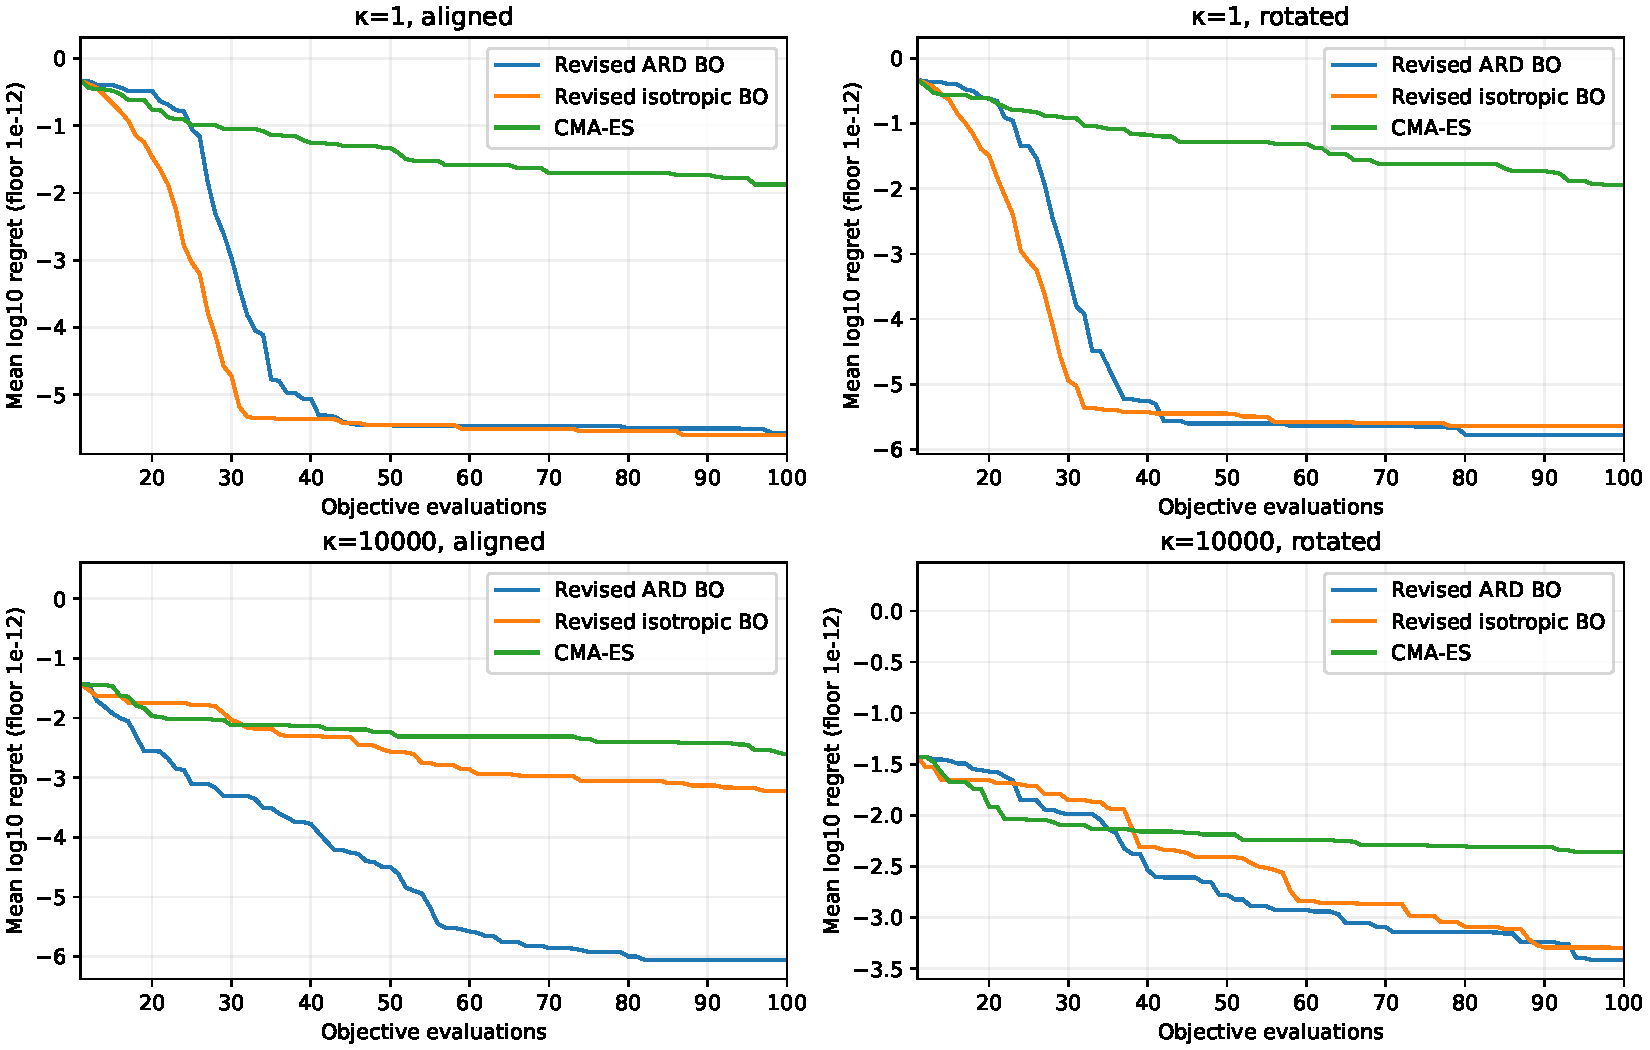
\includegraphics[width=\textwidth]{figures/heldout_convergence.pdf}
\caption{Held-out convergence at 100 calls. Curves average log-regret over
 three instances and two search seeds each; lower is better. All methods share
 their first 11 observations. Panels have different vertical scales. These
 are evaluation-budget curves, not equal-wall-time comparisons.}
\label{fig:heldout}
\end{figure}

The geometry effect persists: ARD's ill-conditioned rotation effect is
2.645 [2.496, 2.861], approximately 441-fold higher geometric-mean regret.
Its interaction is 2.864 [2.526, 3.205], whereas the isotropic interaction
is $-0.044$ [$-0.141, 0.132$] (Figure~\ref{fig:interaction}). This supports
the coordinate-metric explanation on held-out cases after improving acquisition.

CMA-ES also has a positive interaction, 0.323 [0.226, 0.381], complicating a
claim that only ARD responds to rotation. Its ill-conditioned rotation effect
is 0.253 [$-0.029, 0.443$]. Such finite-sample contrasts do not establish a
violation of distributional rotation invariance: later random proposals are
not coupled through $Q$, and only three instances are represented.
Sphere-control rotation intervals include zero for every method.
\begin{figure}[htbp]
\centering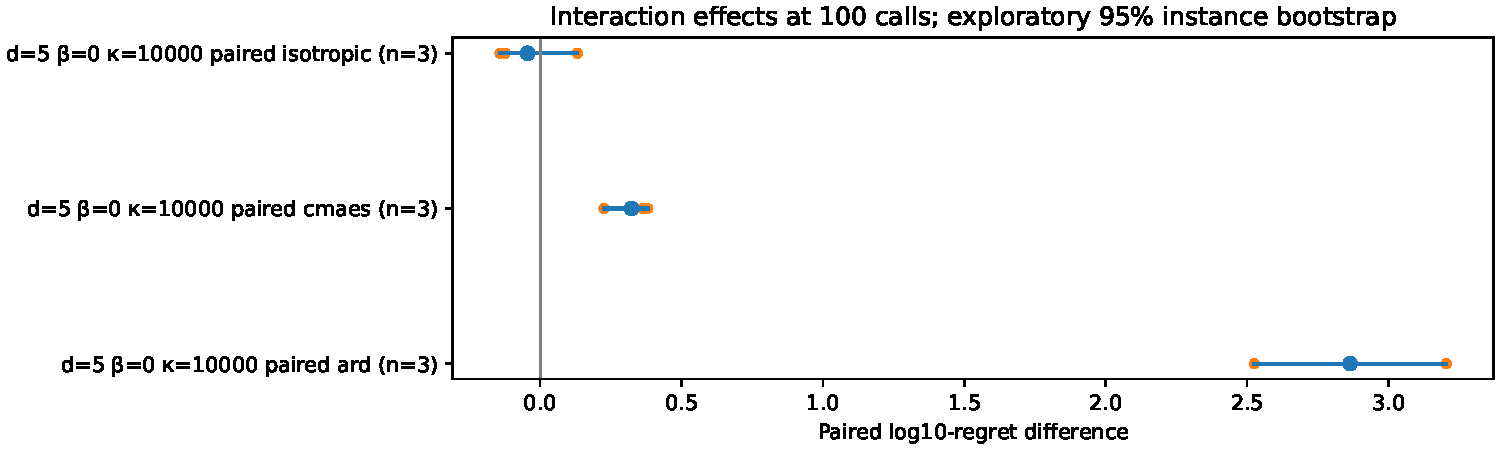
\includegraphics[width=\textwidth]{figures/heldout_interaction.pdf}
\caption{Increase in rotation penalty from $\kappa=1$ to $10000$ at 100 calls.
 ARD and isotropic labels denote revised BO. Orange dots are instance means;
 blue dots and lines are aggregate means and exploratory 95\% instance-bootstrap
 intervals. Positive values indicate a larger penalty at high conditioning.}
\label{fig:interaction}
\end{figure}

\subsection{Computation and the separate timing pilot}
At 100 calls, median search times (IQRs) were 35.87 [27.04, 42.07] seconds
for ARD, 36.37 [29.53, 42.77] for isotropic BO and
0.00436 [0.00425, 0.00448] for CMA-ES. The evaluation-efficiency advantage
therefore costs substantial computation on this cheap objective. These are
machine-specific timings, not an equal-wall-time trial.

The separate pilot below uses only rotated $\kappa=10000$, instance 3,
seed 0. All three fresh runs completed 500 calls and exactly reproduced their
corresponding held-out first-100 input/output pairs. Times are cumulative
within each pilot run; no bootstrap intervals are appropriate.
\begin{center}
\small
\begin{tabular}{lrrrr}
\hline
Method & Regret, 100 & Regret, 500 & Seconds, 100 & Seconds, 500 \\
\hline
ARD BO & $5.76\times10^{-4}$ & $1.11\times10^{-7}$ & 27.44 & 319.43 \\
Isotropic BO & $8.95\times10^{-4}$ & $5.20\times10^{-7}$ & 24.21 & 280.87 \\
CMA-ES & $3.78\times10^{-3}$ & $6.30\times10^{-5}$ & 0.00493 & 0.01944 \\
\hline
\end{tabular}
\end{center}
Five times the evaluation budget required approximately 11.6 times the elapsed
time for both BO kernels and 3.94 times for CMA-ES. ARD spent 56.88 seconds
fitting and 262.54 selecting candidates; isotropic BO spent 22.83 and 258.02
seconds respectively. Objective evaluation took under 0.01 seconds per run.
Both BO variants retained lower regret at 500 calls here, but this single case
does not establish a replicated 500-call ranking. Their late plateaus despite
zero random fallbacks also show that removing one failure mechanism does not
guarantee continued progress.

\section{Limitations and conclusion}
The experiment supports two related explanations. First, acquisition arithmetic
and candidate coverage can materially limit a GP-based optimiser even when
its surrogate still offers useful guidance. Second, after addressing those
issues, ARD retains a much larger conditioning--rotation interaction than
isotropic BO, consistent with its diagonal coordinate metric. The CMA-ES
counterexample and finite instance sample prevent a stronger invariance claim.

The scope is five-dimensional, noiseless, single-basin quadratics. Three
instances per repeated study give limited uncertainty estimates, and GP
warnings remain frequent (Appendix~\ref{app:diagnostics}). No claim is made
about noise, multimodality, high dimensions, parallel workers or general
algorithm superiority. The earlier and held-out cohorts differ in both
instances and budget and cannot be pooled to estimate an acquisition effect.
The ablation shares an instance with development; held-out validation reduces,
but does not eliminate, concerns about selecting an implementation for this family.
CMA-ES did not receive a comparable acquisition-style tuning study, so the
revised comparison evaluates these selected configurations, not equally tuned
algorithm families.

For these tested conditions, revised BO uses a small evaluation budget well,
while CMA-ES has much lower computation cost. ARD's strength on aligned narrow
valleys does not transfer unchanged to rotated valleys. Algorithm choice must
therefore account for geometry, acquisition implementation and the relative
costs of objective calls and optimiser overhead. More instances, dimension and
quartic checks, and equal-wall-time or expensive-objective experiments are useful
future extensions; they are not completed evidence in this report.

\clearpage
\begin{thebibliography}{9}

\bibitem{bbob}
N.~Hansen, S.~Finck, R.~Ros, and A.~Auger.
\newblock \emph{Real-Parameter Black-Box Optimization Benchmarking 2009:
Noiseless Functions Definitions}.
\newblock INRIA Research Report RR-6829, 2009.
\newblock Online presentation:
\url{https://coco-platform.org/testsuites/bbob/overview.html}.

\bibitem{hansen}
N.~Hansen.
\newblock \emph{The CMA Evolution Strategy: A Tutorial}.
\newblock arXiv:1604.00772, 2016; revised 2023.
\newblock \url{https://arxiv.org/abs/1604.00772}.

\bibitem{frazier}
P.~I.~Frazier.
\newblock \emph{A Tutorial on Bayesian Optimization}.
\newblock arXiv:1807.02811, 2018.
\newblock \url{https://arxiv.org/abs/1807.02811}.

\bibitem{pycma}
N.~Hansen and contributors.
\newblock \emph{pycma}, version 4.5.0.
\newblock \url{https://pypi.org/project/cma/4.5.0/}.

\bibitem{logei}
S.~Ament, S.~Daulton, D.~Eriksson, M.~Balandat, and E.~Bakshy.
\newblock \emph{Unexpected Improvements to Expected Improvement for Bayesian Optimization}.
\newblock NeurIPS, 2023. \url{https://arxiv.org/abs/2310.20708}.


\end{thebibliography}
\clearpage
\appendix
\section{Validation, ablation and diagnostics}
\label{app:validation}\label{app:ablation}\label{app:diagnostics}
All seven benchmark checks passed. Landscape validation covered 180 settings
across dimensions 2, 5 and 10, three conditioning levels, both supported
shapes and ten instances. Maximum rotation-equivalence error was
$1.95\times10^{-14}$ and relative condition-number error $1.16\times10^{-12}$.
Quartic and dimension extensions were validated mathematically but were not
part of the optimisation comparisons. Further checks cover acquisition values,
feasibility, budgets, reproducibility, stopping, pairing, bootstrap and resume.

The complete ablation below reports 100-call regret on instance/run 0.
``Local'' uses mixed candidates; ``Both'' combines them with log-EI.
Model settings and budgets are fixed. Additional local draws change later
random streams; frozen-model audits instead clone the candidate RNG.
\begin{center}
\small
\resizebox{\textwidth}{!}{%
\begin{tabular}{lrlrrrr}
\hline
Kernel & $\kappa$ & Orientation & Baseline & Log-EI & Local & Both \\
\hline
ard & 1 & aligned & 0.000381 & 3.14e-05 & 1.98e-06 & 3.06e-06 \\
ard & 1 & rotated & 0.000155 & 0.000227 & 1.65e-06 & 2.15e-06 \\
ard & 10000 & aligned & 4.28e-06 & 1.04e-07 & 8.12e-07 & 1.33e-07 \\
ard & 10000 & rotated & 0.000254 & 0.00016 & 0.000497 & 4.26e-05 \\
isotropic & 1 & aligned & 0.000896 & 5.3e-06 & 3.69e-06 & 9.66e-07 \\
isotropic & 1 & rotated & 0.000102 & 4.12e-05 & 4.49e-06 & 3.64e-06 \\
isotropic & 10000 & aligned & 0.000579 & 0.000258 & 0.000103 & 0.000347 \\
isotropic & 10000 & rotated & 0.00062 & 0.000428 & 0.000352 & 0.000295 \\
\hline
\end{tabular}}
\end{center}

Neither revised BO kernel used random fallbacks in the held-out study
(2,136 proposals each). ARD had 187 failed SLSQP exits and 2,006 warned GP
fits; isotropic BO had 153 failed exits and 1,579 warned fits. Each kernel
attempted 21,360 refinements. Warnings count fits with at least one warning,
not failed runs. Feasible pool candidates remain eligible after refinement
failure. CMA-ES rejected 86 outside-ball proposals, charging time but no calls.
All 179 study runs reached their budgets; this does not mean every internal
numerical optimisation converged.

The repository retains full diagnostic curves, warning records and numerical
results. All code uses functions and dictionaries in
\path{code/prepare_benchmark.py}. Raw records include observations, timings,
settings, versions and source fingerprints. All 75 held-out/pilot records were
reused successfully in resume checks; 136 protected original artifacts retain
their checksums. The README separates saved-data verification from fresh
experiment reproduction. Early implementation pilots are excluded from the
reported comparisons. The full study record is \path{report/comparison.md}.
\end{document}
